\documentclass{../../oss-handout}
\usepackage{titlesec}
\usepackage{tikz}
\usepackage{newtxtext,newtxmath}

\setlength{\parindent}{0pt}
\setlength{\parskip}{2pt}
\setlength{\headheight}{26pt}

\titleformat*{\subsection}{\bfseries}
\titlespacing\subsection{0pt}{10pt plus 4pt minus 4pt}{4pt plus 12pt minus 20pt}

\tikzset{
  >=latex,
}
% Set the page style for the document
\pagestyle{plain}

% Course & handout information
\renewcommand{\institution}{Meritus Academy}
\renewcommand{\coursetitle}{AP Physics 2}
\renewcommand{\term}{Updated: Fall 2022}
\title{Beat Frequency}
\author{Dr.\ T.\ Leung}
\date{\today}

\begin{document}
\thispagestyle{title}
\gentitle

Beats are generated when two waves of different frequencies both constructive
and destructively interfere with each other. For illustration, consider two
one-dimensional waves of frequencies $f_1$ and $f_2$ with equal amplitude $A$
moving in the same medium, as shown Figure~\ref{component-waves}.
\begin{figure}[ht]
  \centering
  \begin{tikzpicture}
    \begin{scope}[->]
      \draw (0,0) --(15.5,0) node[right]{$x$};
      \draw (0,-2) -- (0,2) node[right]{$y$};
      \draw[very thick] (3,2)--(5,2) node[right]{Direction of wave};
    \end{scope}
    \draw (.1,1.5)--(-.1,1.5) node[left]{$A$};
    \draw (.1,-1.5)--(-.1,-1.5) node[left]{$-A$};
    \begin{scope}[smooth,samples=200,domain=0:15,thick]
      \draw[cyan] plot(\x,{1.5*sin(700*\x)});
      \draw[magenta] plot(\x,{1.5*sin(770*\x)});
    \end{scope}
  \end{tikzpicture}
  \caption{Two 1D component waves with different frequencies and identical
    amplitudes moving in the same medium}
  \label{component-waves}
\end{figure}

As the two waves are moving in the same medium (and therefore the same wave
speed), the wavelengths are, correspondingly,
\begin{displaymath}
  \lambda_1=\frac\varv{f_1}\quad\text{and}\quad\lambda_2=\frac\varv{f_2}
\end{displaymath}
where $\varv$ is the speed of the wave in the medium.
Figure~\ref{component-waves} show that there are regions where the two waves
are approximately in phase, and therefore will interfere constructively, as
well as regions where the waves are out of phase, and therefore interfere
destructively. From the principle of superposition, the combined waves is,
literally, the sum of the two waves, as shown in Figure~\ref{sum}.
\begin{figure}[ht]
  \centering
  \begin{tikzpicture}
    \begin{scope}[->]
      \draw (0,0)--(15.5,0) node[right]{$x$};
      \draw (0,-2.5)--(0,2.5) node[right]{$y$};
      \draw[very thick] (3,2.5)--(5,2.5) node[right]{Direction of wave};
    \end{scope}
    \draw (.1,2)--(-.1,2) node[left]{$A'$};
    \draw (.1,-2)--(-.1,-2) node[left]{$-A'$};
    \begin{scope}[smooth,domain=0:15,thick]
      \draw[samples=200,violet] plot(\x,{sin(700*\x)+sin(770*\x)});
      \draw[samples=40,dashed] plot(\x,{ 2*cos(35*\x)});
      \draw[samples=40,dashed] plot(\x,{-2*cos(35*\x)});
    \end{scope}
  \end{tikzpicture}
  \caption{Some of two component waves with different frequencies and
    identical amplitude}
  \label{sum}
\end{figure}

Mathematically, it is easy to find the exact function that describes the
superposition of those two waves. At any fixed position $x$: the waves pass
through with the frequencies:
\begin{equation}
  y = y_1 + y_2 = A\left[\sin(2\pi f_1t)+A\sin(2\pi f_2t)\right]
\end{equation}
Using a lesser-known trigonometric identity called the \textbf{product-sum
  identity}\footnote{This identity is not often taught in high-school level
  math courses}, defined as: %, but it nonetheless very useful here:
\begin{equation}
  \sin\alpha+\sin\beta=2\cos\frac{\alpha-\beta}2\sin\frac{\alpha+\beta}2
\end{equation}
the sum of the waves is given by:
\begin{equation}
  y = \underbrace{2A\cos\left[2\pi\frac{f_1-f_2}2t\right]}_{A'(t)}
  \sin\left[2\pi\frac{f_1+f_2}2t\right]
  \label{eq:sum}
\end{equation}
%where $A'(t)$ is defined as:
%\begin{equation}
%  A'(t)=2A\cos\left[2\pi\frac{f_1-f_2}2t\right]
%\end{equation}
The leading term $A'(t)$ is a slow amplitude variation, with a frequency that is
half of the difference between $f_1$ and $f_2$. This amplitude variation
function correspponds to the dashed line in Figure~\ref{sum}. The maximum
amplitude is $2A$, which corresponds to when the two components waves are
perfectly in phase. Since the human ear is sensitive to the intensity of
sound, which scales with the \emph{square} of the amplitude (i.e.\ $A'^2$) 
rather than amplitude itself. The number of times the intensity $I\propto A'^2$
reaches its maximum value is twice as often as amplitude $A'$.
\begin{figure}[ht]
  \centering
  \begin{tikzpicture}[yscale=.8]
    \begin{scope}[->]
      \draw (0,0)--(15.5,0) node[right]{$x$};
      \draw (0,0)--(0,4.5) node[right]{$I$};
      \draw[very thick] (3,4.3)--(5,4.3) node[right]{Direction of wave};
    \end{scope}
    \draw (.1,4)--(-.1,4) node[left]{$I_\text{max}$};
    \draw[domain=0:15,thick,smooth,samples=100,green!70!black]
    plot(\x,{(4*cos(35*\x)^2});
  \end{tikzpicture}
  \caption{The intensity of of the sum of the  two component waves with
    different frequencies and identical amplitude}
  \label{square}
\end{figure}

The variation of the intensity function creates a pulsation of sound, called a
\emph{beat}. Its frequency, called the \textbf{beat freqeuncy} $f_\text{beat}$,
is \emph{twice} the frequency of $A'$:
\begin{equation}
  \boxed{f_\text{beat}=|f_1-f_2|}
\end{equation}
A second sinusoidal term in Equation~\ref{eq:sum} shows a rapid displacement
variation. This part of the combined wave function has a frequency that is the
average of the two component waves, and its called the \textbf{perceived
  frequency}:
\begin{equation}
  \boxed{f_\text{perceived}=\frac{f_1+f_2}2}
\end{equation}
\end{document}
